\documentclass{beamer}

%% Tema y configuraciones (misma anatomía de mis otros cursos)
\usetheme{Boadilla}
\usecolortheme{default}
\setbeamertemplate{navigation symbols}{}
\usepackage[utf8]{inputenc}
\usepackage[T1]{fontenc}
\usepackage{xcolor}
\usepackage{graphicx}
\usepackage{booktabs}
\usepackage{array}
\usepackage{colortbl}
\hypersetup{
    colorlinks=true,
    linkcolor=.,
    urlcolor=blue,
    citecolor=.,
}

%% Colores de apoyo (los mismos de la semana 5)
\definecolor{verdeok}{RGB}{39,124,74}
\definecolor{rojoal}{RGB}{198,40,40}
\definecolor{naranjal}{RGB}{230,126,34}
\definecolor{grisclaro}{RGB}{242,243,246}
\definecolor{azulcaso}{RGB}{28,60,120}

%% Encabezado
\title[06327-ECO]{Analítica para los negocios \\ 06327-ECO}
\subtitle{Semana 11: El torneo de clasificadores --- ¿quién se va de Cóndor?}
\author{Eduard F. Martínez González, Ph.D.}
\institute[]{Departamento de Economía, Universidad Icesi}
\date{\textcolor{rojoal}{[fecha por definir]}}

%%=================================================
\begin{document}

\begin{frame}
\titlepage
\end{frame}

%%=================================================
\begin{frame}{Objetivo de la sesión}
\small
La semana pasada se juzgaron reglas escritas a mano. Hoy la máquina \textbf{escribe sus propias reglas} --- y compite contra la del EDA, en el mismo sobre sellado.

\vspace{0.15cm}
\begin{itemize} \setlength{\itemsep}{0.16cm}
  \item Un árbol de dos preguntas, comprobado a mano.
  \item El árbol sin frenos y la poda: la validación cruzada como juez que no abre el sobre.
  \item Quinientos árboles votando, su juez gratis y su perilla.
  \item Toda cifra del examen, con su margen.
\end{itemize}

\vspace{0.15cm}
\begin{block}{La idea que gobierna la sesión}
El mejor modelo no es el que más acierta en general, sino el que \textbf{mejor sirve a la decisión}: a quién llama Growth con el cupo que tiene.
\end{block}
\end{frame}

%%=================================================
\begin{frame}{¿Dónde estamos en el curso?}
\small
\begin{itemize} \setlength{\itemsep}{0.22cm}
  \item \textbf{Semana 6:} el EDA --- recencia y sesiones separan a los que se van.
  \item \textbf{Semana 10:} el juicio --- la regla del EDA encuentra a 151 de 354 con 278 llamadas; en accuracy empata con no hacer nada.
  \item \textbf{Semana 11 (hoy):} el entrenamiento --- árboles y bosques, con la tabla del líder de la semana 10 como vara.
\end{itemize}

\vspace{0.2cm}
\begin{block}{Lo que cambia hoy}
Las reglas ya no las escribe el analista: las aprende el modelo, y la validación cruzada decide cuánto dejarlo aprender.
\end{block}
\end{frame}

\begin{frame}[noframenumbering]{Roadmap}
\tableofcontents
\end{frame}

%%=================================================
\section{La vara y la base}

\begin{frame}[noframenumbering]{Roadmap}
\tableofcontents[currentsection]
\end{frame}

\begin{frame}{La pregunta de hoy, con presupuesto}
\small
\begin{block}{La misión de Growth}
``La regla del EDA encuentra a 151 de cada 354 clientes que se van. Tenemos cupo para unas \textbf{280 llamadas por cada 1.600 clientes}. ¿Un modelo entrenado encuentra más con ese cupo?''
\end{block}

\vspace{0.15cm}
\centering
\footnotesize
\textbf{La tabla del líder que dejó la semana 10} (test de 1.600; se van 354)
\vspace{0.05cm}

\begin{tabular}{lrrc}
\toprule
Regla & Llamadas & Encontrados & Accuracy \\
\midrule
Nadie abandona & 0 & 0 & 0,779 ± 0,021 \\
\rowcolor{grisclaro} \textbf{Regla del EDA} & 278 & 151 & 0,794 ± 0,020 \\
Memorizador & 86 & 26 & 0,757 ± 0,021 \\
\bottomrule
\end{tabular}
\end{frame}

\begin{frame}{Paso 1 · ¿Con qué columnas se entrena?}
\small
De las 29 columnas de \texttt{base\_clientes}, salen tres tipos:
\vspace{0.1cm}

\centering
\scriptsize
\begin{tabular}{lll}
\toprule
Columna & Por qué sale & Criterio \\
\midrule
\texttt{gasto\_proximo\_trim} & se conoce después del corte & fuga (semana 10) \\
\texttt{departamento} & 12 ciudades, 12 combinaciones & repite a \texttt{ciudad} \\
\texttt{duracion\_sesion\_promedio} & vacía sin sesiones & ya está en las sesiones \\
\texttt{csat\_promedio} & vacía sin tickets & ya está en los tickets \\
\texttt{score\_buro} & vacía sin crédito & ya está en \texttt{tiene\_credito} \\
\bottomrule
\end{tabular}
\raggedright
\small
\pause
\vspace{0.25cm}
\begin{alertblock}{Hallazgo 1}
Quedan \textbf{22 predictoras} y el mismo sobre de la semana 10 (6.400 en train, 1.600 en test): la comparación con la tabla del líder es justa. Y el bosque no acepta vacíos: los ``no aplica'' se resuelven con criterio, no con la media.
\end{alertblock}
\end{frame}

%%=================================================
\section{El árbol}

\begin{frame}[noframenumbering]{Roadmap}
\tableofcontents[currentsection]
\end{frame}

\begin{frame}{Paso 2 · ¿Qué pregunta haría la máquina?}
\small
\begin{columns}[T]
\column{0.5\textwidth}
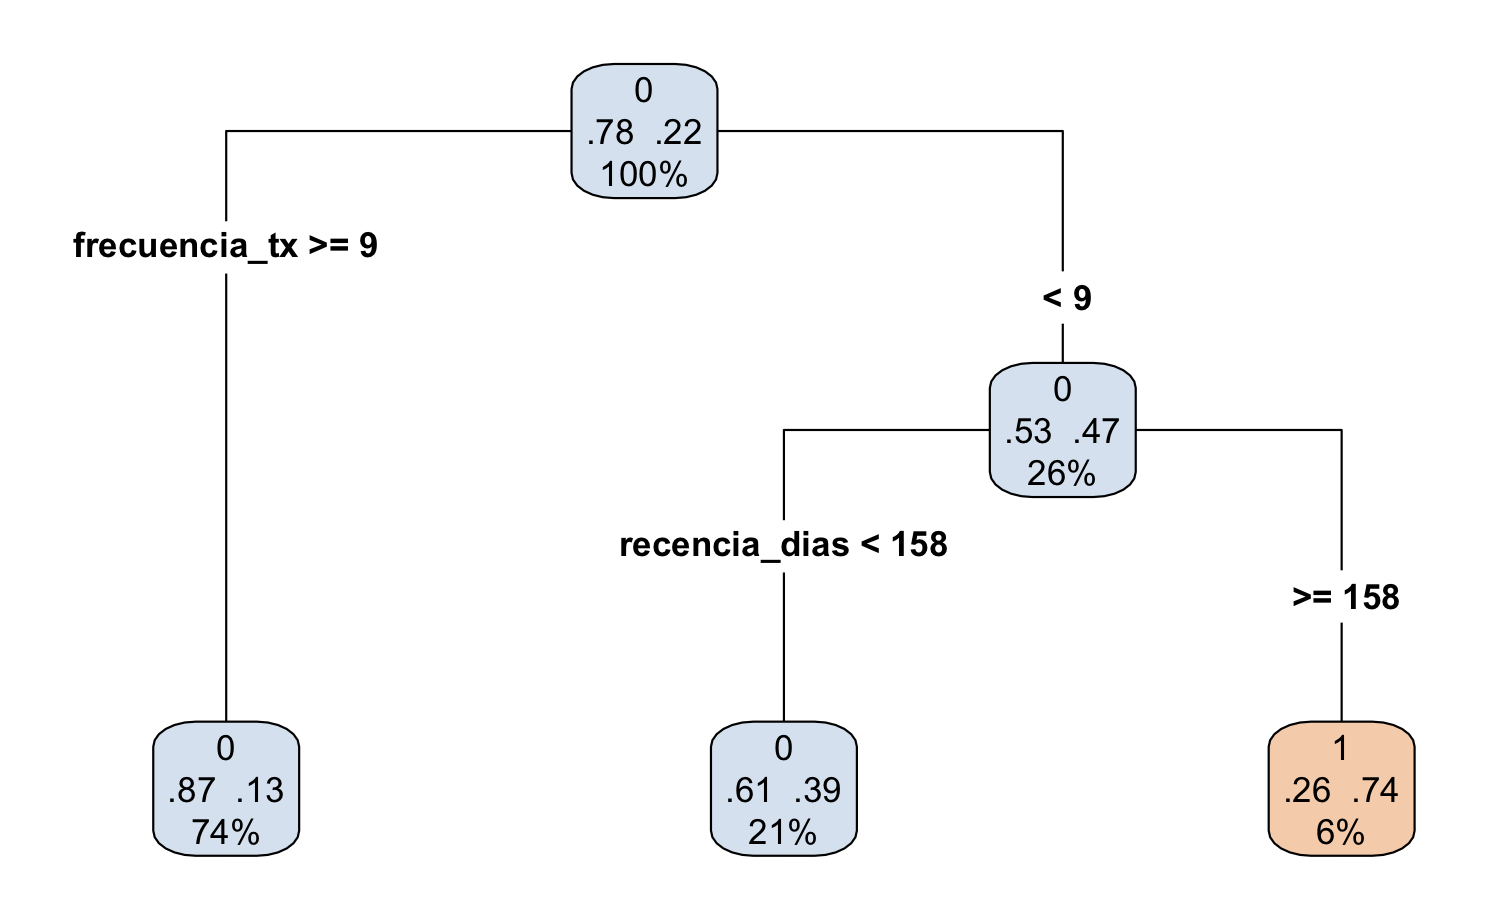
\includegraphics[width=0.93\textwidth]{pic/fig_s11_arbol.png}
\column{0.5\textwidth}
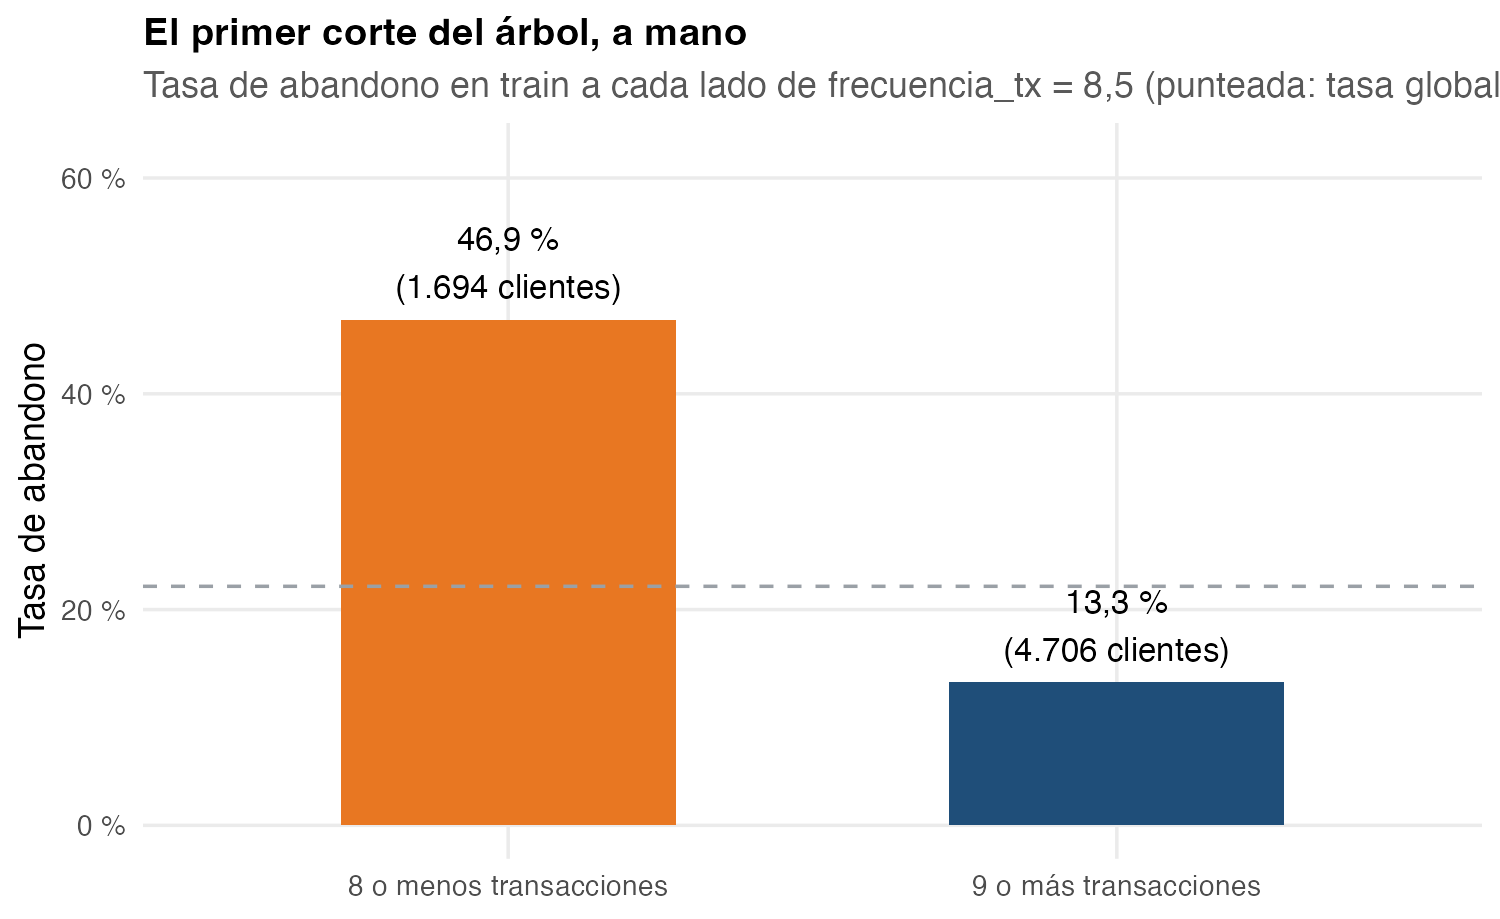
\includegraphics[width=0.93\textwidth]{pic/fig_s11_corte.png}
\end{columns}
\vspace{0.05cm}
\begin{itemize} \itemsep2pt
  \item El árbol prueba todos los cortes de las 22 variables y se queda con el que más separa: \textbf{8 o menos transacciones} (47\,\% se va) contra \textbf{9 o más} (13\,\%).
  \item En test: accuracy \textbf{0,805 ± 0,020}, pero solo 76 llamadas y 59 encontrados (recall \textbf{0,167 ± 0,040}).
\end{itemize}
\pause
\begin{alertblock}{Hallazgo 2}
El árbol hace \textbf{solo} lo que se hizo a mano en la semana 6: comparar tasas por tramo. Repitió la recencia (158 días en vez de 90) y cambió sesiones por frecuencia. En accuracy empata con la regla del EDA; a Growth le sirve menos.
\end{alertblock}
\end{frame}

\begin{frame}{Paso 3 · ¿Cuánto árbol es demasiado árbol?}
\small
\begin{columns}[T]
\column{0.58\textwidth}
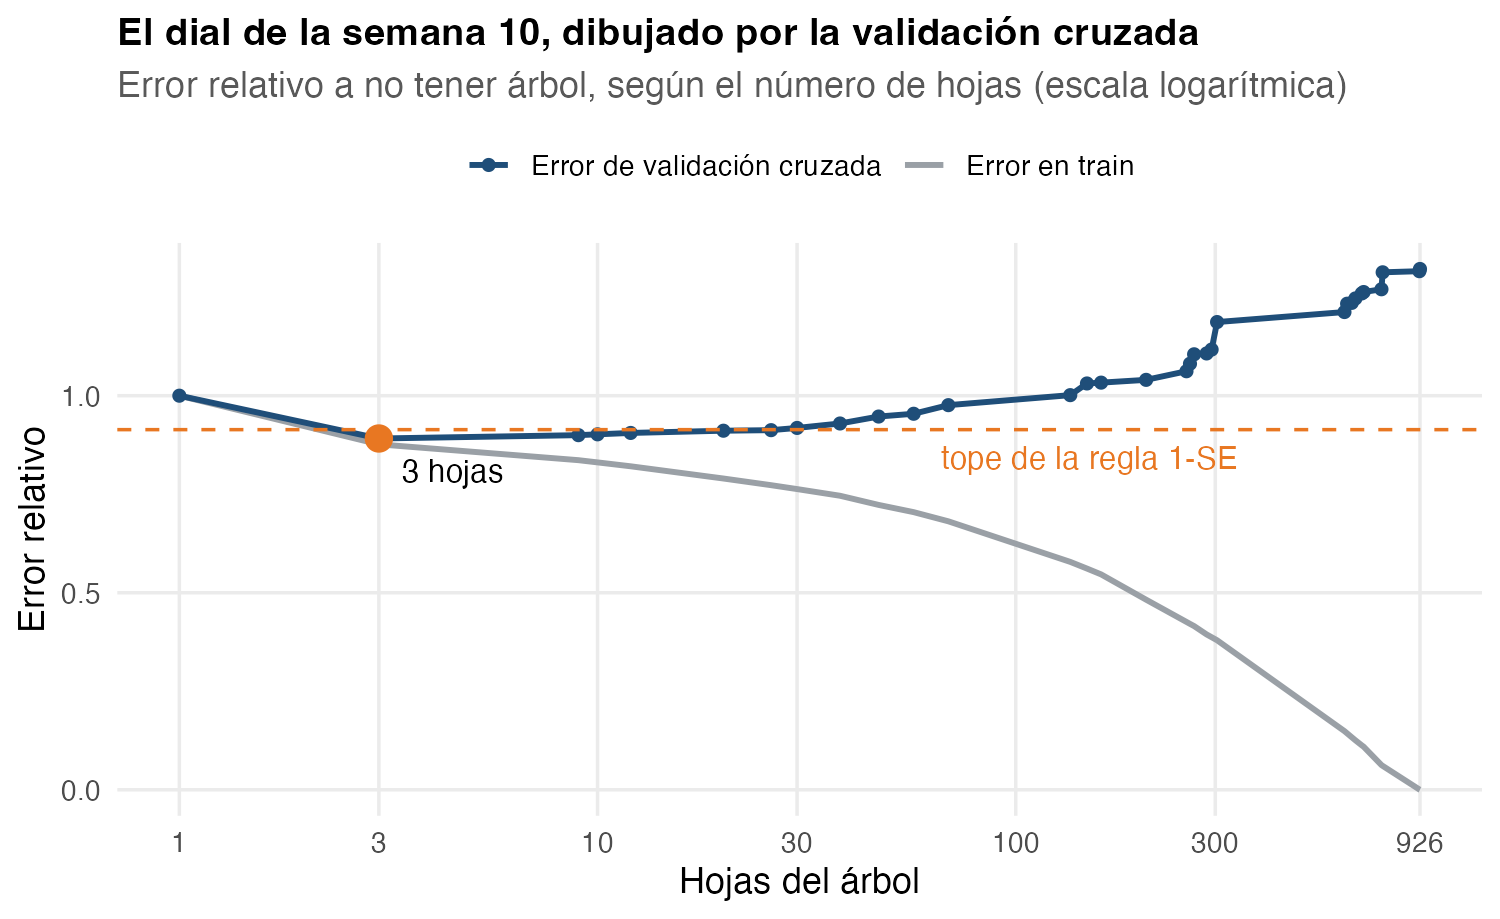
\includegraphics[width=\textwidth]{pic/fig_s11_dial.png}
\column{0.4\textwidth}
\footnotesize
\textbf{El árbol sin frenos} (\texttt{cp = 0,0001}, hojas de un cliente):
\begin{itemize} \setlength{\itemsep}{0.08cm}
  \item \textbf{926 hojas}; train \textbf{100\,\%}; test \textbf{0,729 ± 0,022}, por debajo de no hacer nada.
  \item La validación cruzada: de \textbf{1,00} a \textbf{0,89} con 2 cortes, y sube hasta \textbf{1,32}.
  \item Regla 1-SE: tope 0,89 + 0,02 = 0,91 $\Rightarrow$ \textbf{3 hojas}.
\end{itemize}
\end{columns}
\pause
\vspace{0.1cm}
\begin{alertblock}{Hallazgo 3}
La poda devuelve \textbf{exactamente} el árbol de dos preguntas: la CV confirmó, sin abrir el sobre, que las otras 923 hojas compraban ruido.
\end{alertblock}
\end{frame}

%%=================================================
\section{El bosque y la perilla}

\begin{frame}[noframenumbering]{Roadmap}
\tableofcontents[currentsection]
\end{frame}

\begin{frame}{Paso 4 · ¿Qué gana el bosque votando?}
\small
\begin{columns}[T]
\column{0.55\textwidth}
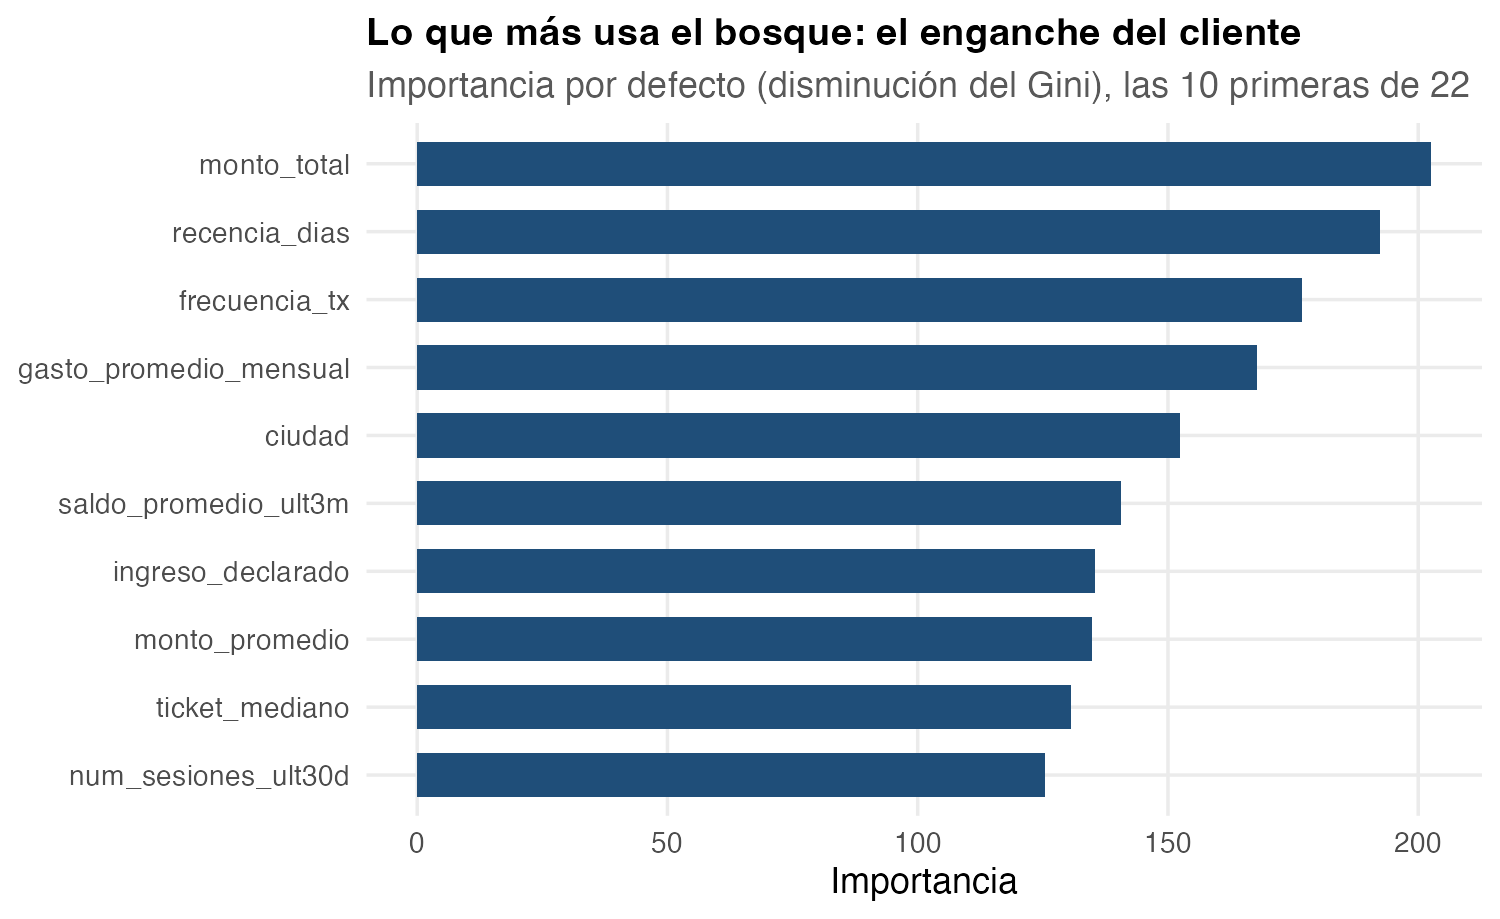
\includegraphics[width=\textwidth]{pic/fig_s11_importancia.png}
\column{0.43\textwidth}
\footnotesize
\begin{itemize} \setlength{\itemsep}{0.08cm}
  \item 500 árboles sobre remuestras de train; en cada corte, 4 variables al azar.
  \item \textbf{Juez gratis} (fuera de la bolsa): error de 19,8\,\%, accuracy \textbf{0,802} sin abrir el sobre.
  \item Test: accuracy \textbf{0,809 ± 0,020} --- la más alta del torneo.
\end{itemize}
\end{columns}
\pause
\vspace{0.1cm}
\begin{alertblock}{Hallazgo 4}
El juez gratis y el examen coinciden. La accuracy más alta\ldots\ \textbf{empata} con el árbol y con la regla del EDA. Lo que más usa el bosque es el enganche del cliente, lo mismo que encontró el EDA.
\end{alertblock}
\end{frame}

\begin{frame}{Paso 5 · ¿A quién llama Growth con su cupo?}
\small
\begin{columns}[T]
\column{0.6\textwidth}
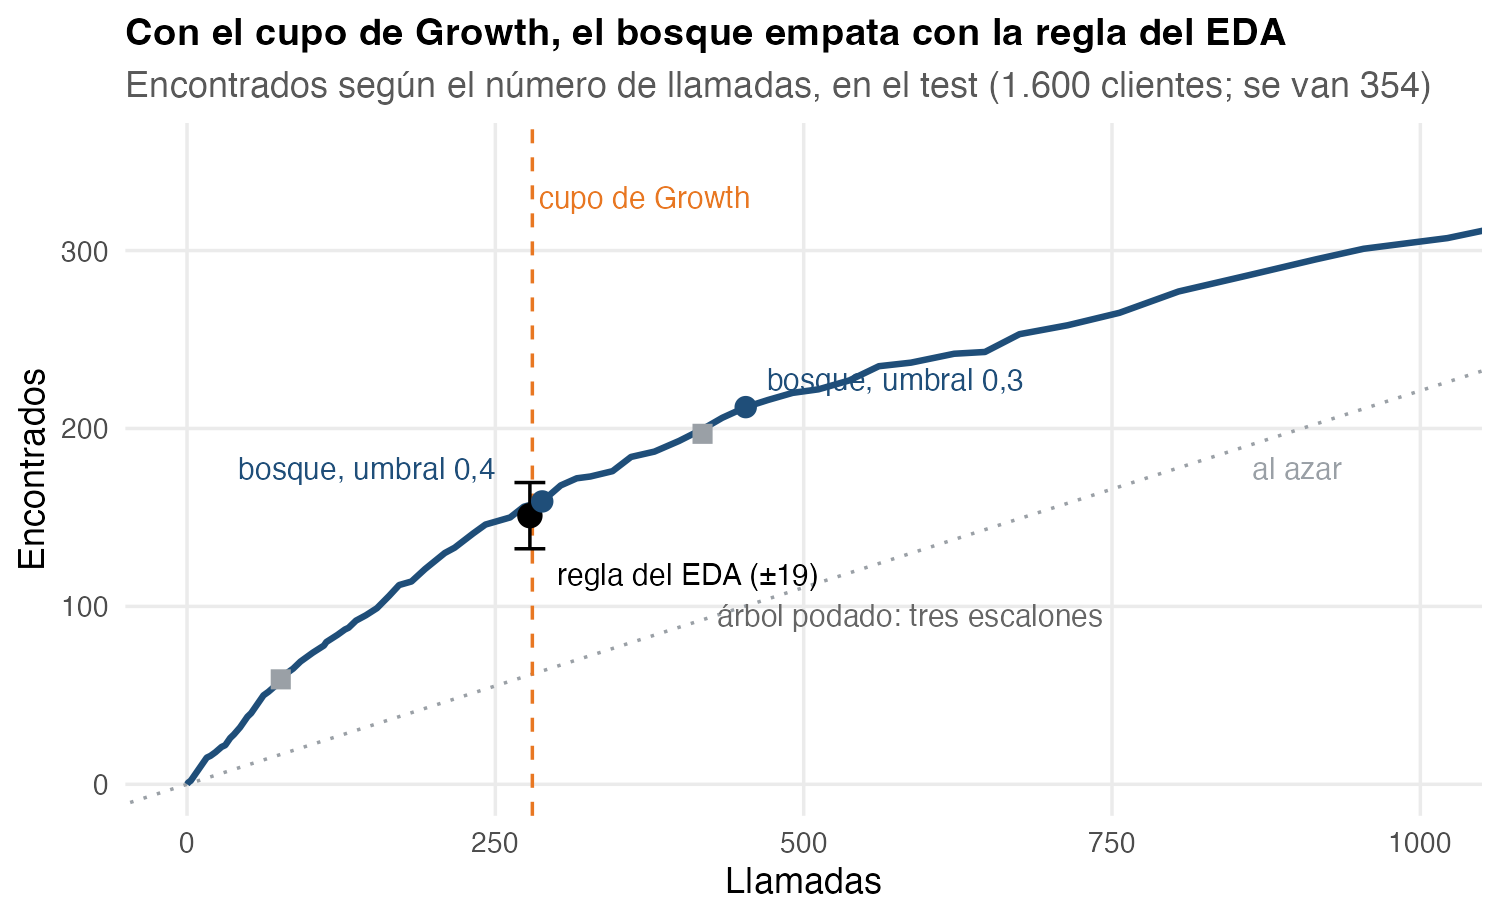
\includegraphics[width=\textwidth]{pic/fig_s11_cupo.png}
\column{0.38\textwidth}
\footnotesize
\begin{itemize} \setlength{\itemsep}{0.08cm}
  \item El bosque da una \textbf{probabilidad}; el umbral la vuelve decisión.
  \item Umbral 0,4: \textbf{288} llamadas, \textbf{159} encontrados.
  \item Regla del EDA: 278 llamadas, 151 encontrados, margen \textbf{±19}.
  \item Umbral 0,3: 453 llamadas, 212 encontrados.
\end{itemize}
\end{columns}
\pause
\vspace{0.1cm}
\begin{alertblock}{Hallazgo 5 --- la lección de la semana}
Con el cupo de Growth, \textbf{empate técnico}. Lo que compra el bosque es \textbf{la perilla}: ordena a los 1.600 por riesgo y deja fijar el cupo. El árbol podado no puede: su perilla salta en tres escalones.
\end{alertblock}
\end{frame}

\begin{frame}{Paso 5 · ¿Y son creíbles esas probabilidades?}
\small
\begin{center}
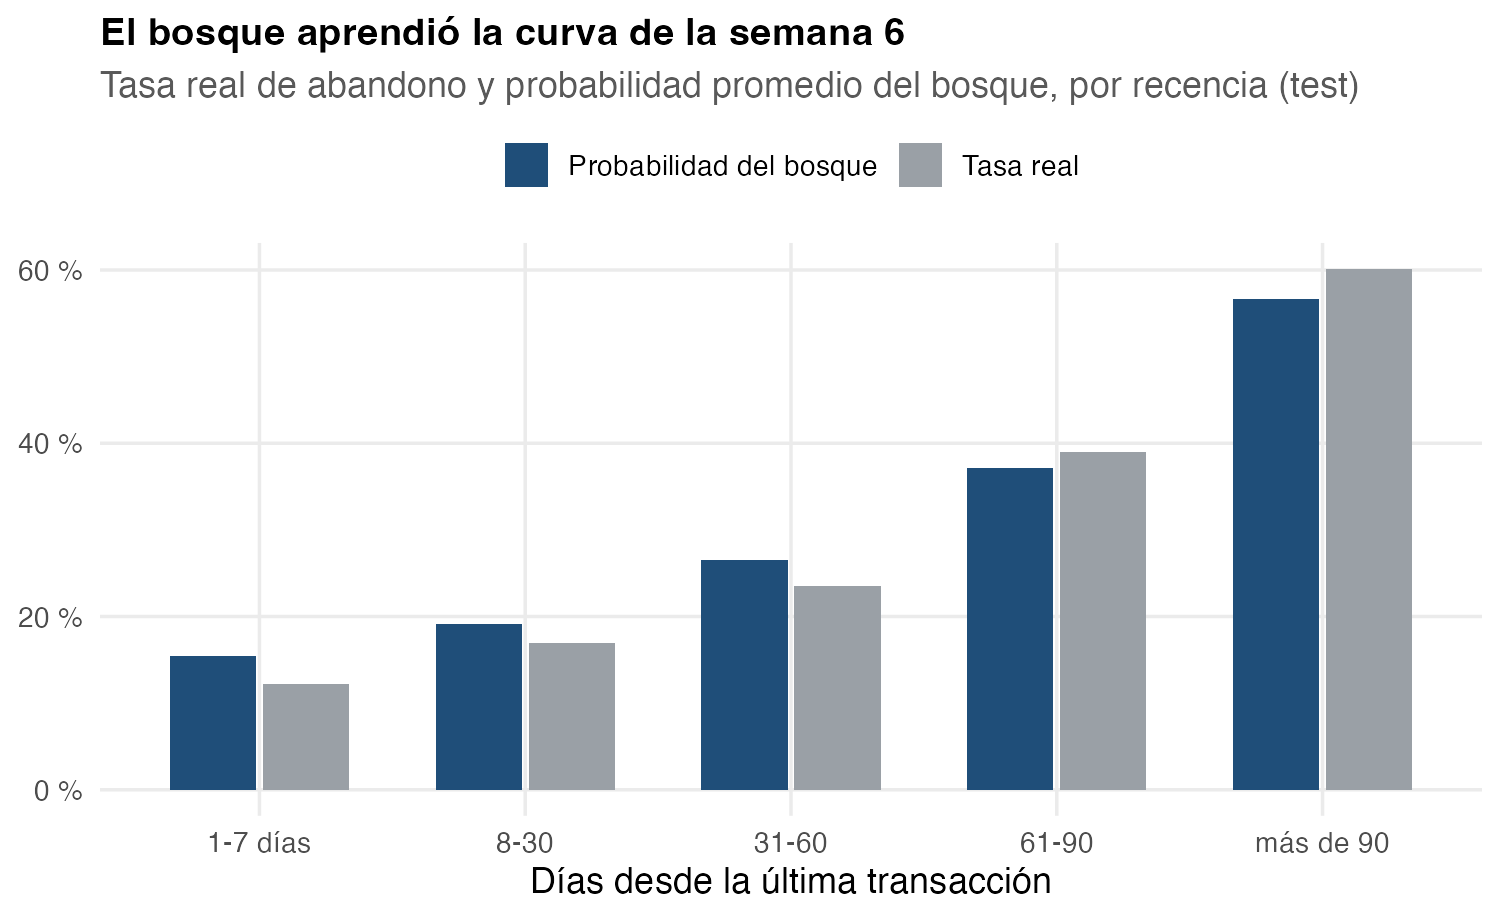
\includegraphics[width=0.66\textwidth]{pic/fig_s11_calibracion.png}
\end{center}
\vspace{-0.2cm}
\begin{itemize} \itemsep2pt
  \item Tasa real por tramo de recencia: de \textbf{12,2\,\%} a \textbf{60,1\,\%}. Probabilidad promedio del bosque: de \textbf{15,4\,\%} a \textbf{56,7\,\%} --- nunca a más de 4 puntos.
\end{itemize}
\begin{block}{La decisión del paso}
Las probabilidades son creíbles y el bosque aprendió la curva de la semana 6: su riesgo sirve para decidir el cupo.
\end{block}
\end{frame}

%%=================================================
\section{Lo que queda}

\begin{frame}[noframenumbering]{Roadmap}
\tableofcontents[currentsection]
\end{frame}

\begin{frame}{La tabla del líder}
\small
\centering
\footnotesize
\textbf{Abandono} (test de 1.600 clientes; se van 354)
\vspace{0.05cm}

\begin{tabular}{lrrc}
\toprule
Regla o modelo & Llamadas & Encontrados & Accuracy \\
\midrule
Nadie abandona & 0 & 0 & 0,779 ± 0,021 \\
\rowcolor{grisclaro} \textbf{Regla del EDA} & 278 & 151 & 0,794 ± 0,020 \\
Memorizador & 86 & 26 & 0,757 ± 0,021 \\
Árbol de dos preguntas & 76 & 59 & 0,805 ± 0,020 \\
Árbol sin frenos & 344 & 132 & 0,729 ± 0,022 \\
Bosque, umbral 0,5 & 164 & 106 & 0,809 ± 0,020 \\
\rowcolor{grisclaro} \textbf{Bosque, umbral 0,4} & 288 & 159 & 0,797 ± 0,020 \\
\bottomrule
\end{tabular}

\raggedright
\small
\pause
\vspace{0.2cm}
\begin{block}{La decisión}
Nadie desbanca a la regla del EDA por más que el margen. El bosque entra como \textbf{colíder}: no porque acierte más, sino porque su riesgo ordena a todos los clientes.
\end{block}
\end{frame}

\begin{frame}{Qué produce un torneo --- y qué no}
\small
\begin{columns}[T]
\column{0.48\textwidth}
\textbf{Produce}
\begin{itemize} \setlength{\itemsep}{0.1cm}
  \item Modelos elegidos por el juez (la CV), no por el examen.
  \item Un riesgo creíble para cada cliente.
  \item Una regla legible (el árbol) y un ordenador fino (el bosque).
\end{itemize}
\column{0.48\textwidth}
\textbf{No produce}
\begin{itemize} \setlength{\itemsep}{0.1cm}
  \item Causas: la importancia dice qué \emph{usó} el bosque, no qué \emph{causa} el abandono.
  \item Más señal que la que hay: con estos datos, el EDA ya había encontrado casi toda.
  \item Clientes que se van por razones que no están en la base.
\end{itemize}
\end{columns}
\end{frame}

\end{document}
